%!TEX encoding = UTF-8 Unicode
\documentclass{lecturenotes}

\setbeamertemplate{footline}[frame number]
\title[Scala introduktion]{Scala for Java developers}
\subtitle{-- A three-hour crash course}
\author{Björn Regnell}
\institute{Dept. of Computer Science, LTH \\ Lund University, Sweden}
\date{2016 April 20}

\begin{document}

\frame{\titlepage}
\frame{\Emph{Agenda}\tableofcontents}

%%% EXPERIENCES

\section[Intro]{Introduction to Scala}

\subsection[What is Scala?]{What is Scala?}

%%
\begin{Slide}{Background}
The aim of Scala: A scalable, pragmatic, real-world language
\begin{multicols}{2}

\begin{itemize}\fontsize{7}{8}\selectfont
\item \href{https://en.wikipedia.org/wiki/Scala_%28programming_language%29}{en.wikipedia.org/wiki/Scala progrogramming language}

\item \Emph{Multi-paradigm:} \Alert{object-oriented, functional, imperative, concurrent}
\item \Emph{Designed by:} \Alert{ Martin Odersky}
\item \Emph{Developer:} \Alert{ EPFL, Lightbend, OSS}
\item \Emph{First appeared:} \Alert{ January 20, 2004}
\item \Emph{Stable release:} \Alert{ 2.11.8 / March 8, 2016}
\item \Emph{Typing:} \Alert{	static, strong, inferred, structural}
\item \Emph{Platform:} \Alert{ 	JVM, JavaScript}
\item \Emph{License:} \Alert{ 	BSD 3-clause}
\item \Emph{File ext:} \Alert{ .scala}

\item \Emph{Official site:} \href{http://www.scala-lang.org/}{www.scala-lang.org/}
\end{itemize}

\columnbreak


\includegraphics[width=0.47\textwidth]{../../img/scala-icon}
\end{multicols}
\end{Slide}

\begin{Slide}{Scala History}\fontsize{9}{11}\selectfont
Heritage: Algol, Modula-2, Simula, Pizza, Java, Beta, OCaml, Haskell, ...\\ Time line:
\begin{itemize}
\item 2004: 1.0, 1.1, 1.2, 1.3
\item 2005: 1.4
\item 2006: 2.0, 2.1, 2.2, 2.3; \Emph{\code{scalac} written in Scala}
\item 2007: 2.4, 2.5, 2.6
\item 2008: 2.7; 
\item 2010: 2.8; \Emph{Play} gets a scala plug-in, \Emph{Akka}
\item 2011: 2.9; \Emph{Typesafe}; \Alert{\code{scala.collection.parallel}}, Play in Scala
\item 2013: 2.10 value classes, implicit classes, string interpolators, \\ \code{Try}, \code{Future}, \code{Promise}, \code{Dynamic}, Akka actors
\item 2014: 2.11; optimizations; 10x faster compilation
\item 2016: 2.12; Java 8, Scala.js, \Emph{Scala Center}@EPFL, \Emph{Lightbend}
\end{itemize}
\href{https://www.artima.com/scalazine/articles/origins_of_scala.html}{[Bill Venners, Frank Sommers]} \\
\href{https://speakerdeck.com/marconilanna/what-is-new-since-programming-in-scala}{[Marconi Lanna]}
\end{Slide}



\subsection[What can you do with Scala?]{What can you do with Scala?}
%%
\begin{Slide}{Scala -- the simple parts}
\fontsize{9}{11}\selectfont
Lecture by \Emph{Martin Odersky}: \href{https://www.youtube.com/watch?v=ecekSCX3B4Q}{www.youtube.com/watch?v=ecekSCX3B4Q}

\begin{multicols}{2}
\fontsize{9}{11}\selectfont
Scala for every-day dev actions:

\begin{enumerate}
\item \Emph{Compose:} everything is a composable \Alert{expression}
\item \Emph{Match:} decompose data with \Alert{pattern}-matching
\item \Emph{Group:} everything can be grouped and \Alert{nested}
\item \Emph{Recurse:} compose at any depth; better loops \code{@tailrec}
\item \Emph{Abstract:} functions are objects
\item \Emph{Aggregate:} collections aggregate \& \Alert{transform} data
\item \Emph{Mutate:} local, private mutability to optimize perf.
\end{enumerate}

\columnbreak

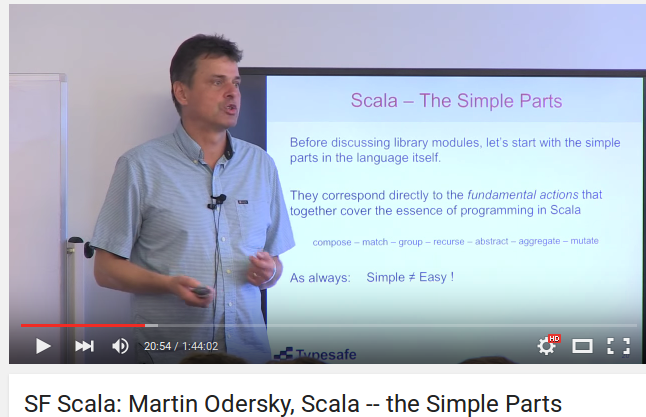
\includegraphics[width=0.62\textwidth]{img/odersky}

\end{multicols}
\end{Slide}

\subsection[Scala versus Java]{Similarities and differences between Scala and Java}

\begin{Slide}{Some similarities between Scala and Java}
\begin{itemize}
\item Both are object-oriented and imperative
\item Both are statically typed (\code{~} 100 times faster than Python)
\item Both have C-like block syntax \code+{ }+
\item Both have lambdas (Java 8)  
\item Both run on the JVM
\item Both can execute each other's byte code
\end{itemize}
\end{Slide}


\begin{Slide}{Some differences between Scala and Java}\footnotesize
\begin{itemize}
\item Scala is a more ''pure'' OO language: \\ instances of \Emph{\code{Int, Double, Char}}, etc. are \Alert{real objects} 
\item Scala is a more advanced functional language: \\ easy to transform immutable data in functional collections
\item Scala unifies OO and functional programming: \\ functions are objects with an \code{apply}-method
\item singelton \code{object} instead of Java's \code{static}

\item Some syntax differences: \pause
\begin{itemize}\fontsize{8}{9}\selectfont
\item semicolons are inferred; newline btw statements is enough
\item no need for \code{return} as blocks are values
\item Type \emph{after} names and colon: \code{val name: String = "Kim"}
\item generic types in \code{[T]} instead of \code{<T>}
\item Five types of members: \code{def, val, lazy val, var, type}
\\ Methods: \code{def isChild: Boolean = age < 18} 
\\ Immutable fields: \code{val gender = "Female"} 
\\  Delayed init: \code{lazy val r = List.fill(1000)(math.random)} 
\\  Mutable fields: \code{var age: Int = 42} 
\\  Type alias: \code{type Matrix = Map[Int, Map[Int, String]]}
\end{itemize}


\end{itemize}

\end{Slide}

\begin{Slide}{Classes in Java and Scala}
\vspace{-1.5em}
\begin{multicols}{2}

\javainputlisting{code/JPerson.java}

\columnbreak

\pause

\scalainputlisting{code/SPerson.scala}

\pause

\scalainputlisting{code/Person.scala}

\end{multicols}

\end{Slide}

\section[Live Scala coding]{Live Scala coding}

\begin{Slide}{Live coding: code-along}
Start the REPL:
\begin{REPL}
$ scala
Welcome to Scala 2.11.8 (Java HotSpot(TM) VM, Java 1.8.0_66).
Type in expressions for evaluation. Or try :help.

scala> case class Person(name: String, age: Int = 42)
defined class Person

scala> Person("Björn", 48)
res0: Person = Person(Björn,48)

scala> Person("Kim")
res1: Person = Person(Kim,42)
\end{REPL}

\end{Slide}


\begin{Slide}{Functions are first-class values; Try this in REPL:}
\begin{REPL}[basicstyle=\color{white}\ttfamily\fontsize{8.5}{10}\selectfont]
def öka(i: Int) = i + 1

val nums = Vector(1, 2, 3, 4, 42)

nums.map(öka)

nums.map(i => i + 1)

nums.map(_ + 1)

def mappa(xs: Vector[Int], f: Int => Int) = xs.map(f)  

mappa(nums, öka)

def upprepa(n: Int)(block: => Unit) = for (i <- 1 to n) block
\end{REPL}

\end{Slide}

\section[Overview of new course at LTH]{Overview of new course at LTH: EDAA45 Scala + Java}

\begin{Slide}{Overview of new LTH Course EDAA45 (was EDA016)}
Open Source project, on-going course dev: \url{https://github.com/lunduniversity/introprog} \\ \vspace{1em}

\noindent\resizebox{0.8\columnwidth}{!}{\fontsize{8}{10}\selectfont
\begin{tabular}{l|l|l|l}
\textit{W} & \textit{Modul} & \textit{Övn} & \textit{Lab} \\ \hline \hline
W01 & Introduktion         & expressions & kojo            \\
W02 & Kodstrukturer        & programs    & --              \\
W03 & Funktioner, Objekt   & functions   & simplewindow    \\
W04 & Datastrukturer       & data        & textfiles       \\
W05 & Vektoralgoritmer     & vectors     & cardgame        \\
W06 & Klasser, Likhet      & classes     & shapes          \\
W07 & Arv, Gränssnitt      & traits      & turtlerace-team \\
KS  & KONTROLLSKRIVN.      & --          & --              \\
W08 & Mönster, Undantag    & matching    & chords-team     \\
W09 & Matriser             & matrices    & maze            \\
W10 & Sökning, Sortering   & sorting     & surveydata-team \\
W11 & Scala och Java       & scalajava   & scalajava-team  \\
W12 & Trådar, Web, Android & threads     & life            \\
W13 & Design               & Uppsamling  & Inl.Uppg.       \\
W14 & Tentaträning         & Extenta     & --              \\
T   & TENTAMEN             & --          & --              \\
\end{tabular}

}
\end{Slide}


\section[Workshop]{Workshop: Exercises in Scala}

\begin{Slide}{Workshop: Exercises in Scala}
Test our \Alert{DRAFT} exercises in Scala:  \\ 
\href{https://github.com/lunduniversity/introprog/blob/master/compendium/exercises.pdf}{\footnotesize github.com/lunduniversity/introprog/blob/master/compendium/exercises.pdf}
 \\ 
\Emph{Feedback welcome!}
\begin{enumerate}\fontsize{8}{10}\selectfont
\item Övning \Emph{\code{expressions}}:  skim and jump to 17 stringinterp., 19 if, 20 for, 21 foreach, 22 while, 35 scaladoc, 36 stringinterp.
\item Övning \Emph{\code{programs}}: 1 Range, 2 Array, 3 Vector, 4 for-expr, 5 map, 6 foreach, 9 hello app, 11 a)-c) sumbug, 13 name space
\item Övning \Emph{\code{functions}}: 1--15, 18, 19, 21--23 
\item Övning \Emph{\code{data}}: 1--4, 6--18, 20,  21, 27, 28
\item Övning \Emph{\code{sequences}} (only half-ready) -- 1, 4, 7  
\end{enumerate}

If time permits: \\ We will close with live coding of some more advanced aspects

\end{Slide}

\end{document}
